\chapter{High Multiplicity Jets at \texttt{ATLAS}}
\label{chap:ATLAS}

Show the ATLAS pure jets analysis and talk a bit about the issues with running the damn thing.  Talk about the conclusions about BFKL-like dynamics

\chapter{The $W^\pm$ to $\zg$ Ratio at \texttt{ATLAS}}
\label{chap:WZRatio}

Compare HEJ Z+Jets to NJet (NLO predictions) and MadGraph (LO predictions)

\chapter{$\zg$+Jets at 100TeV}
\label{chap:100TeV}

	Talk about the FCC movement and the effect we expect the resummation will have at these energies

	\begin{figure}[h]
		\centering
		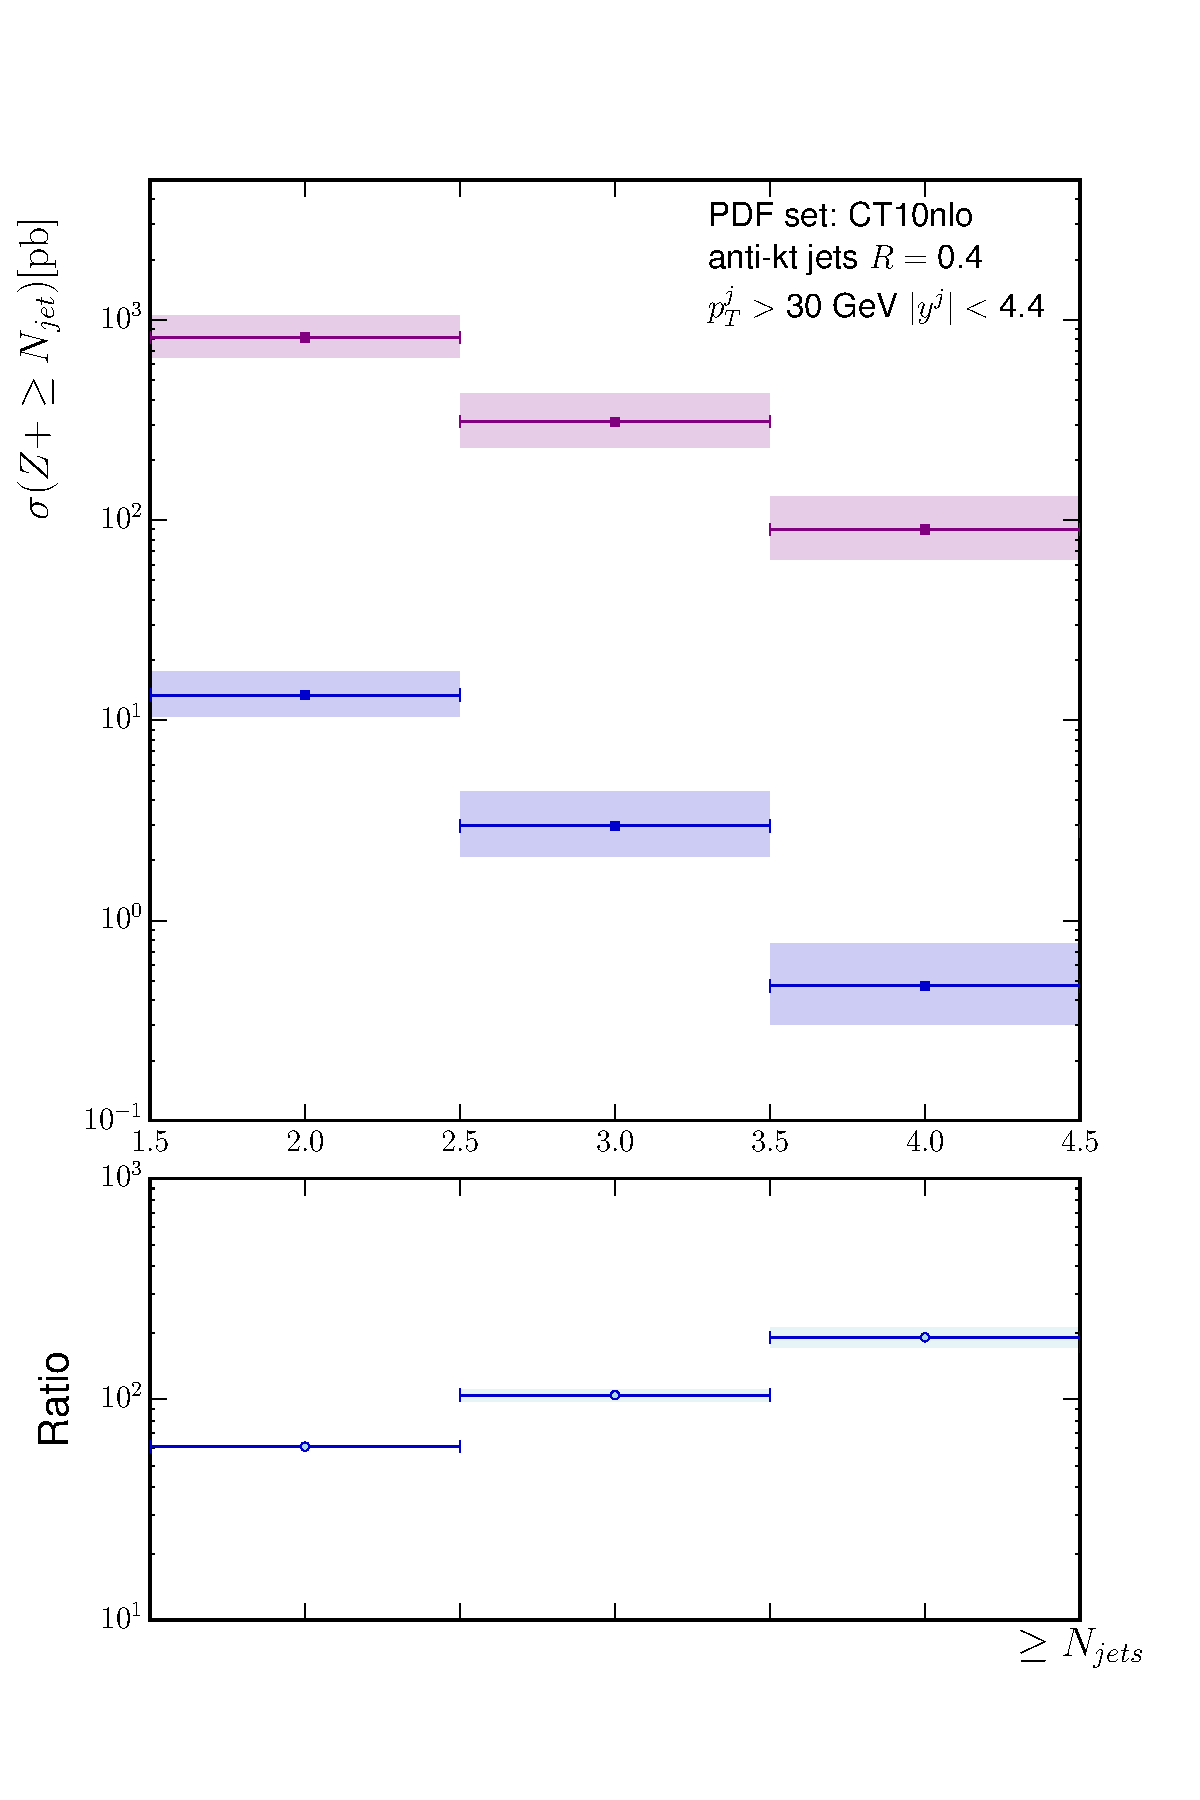
\includegraphics[width=0.8\linewidth]{Figures/ATLAS_Z_100TeV_2a.pdf}
		\caption{2a}
		\label{fig:emissionsites}
	\end{figure}

	\begin{figure}[h]
		\centering
		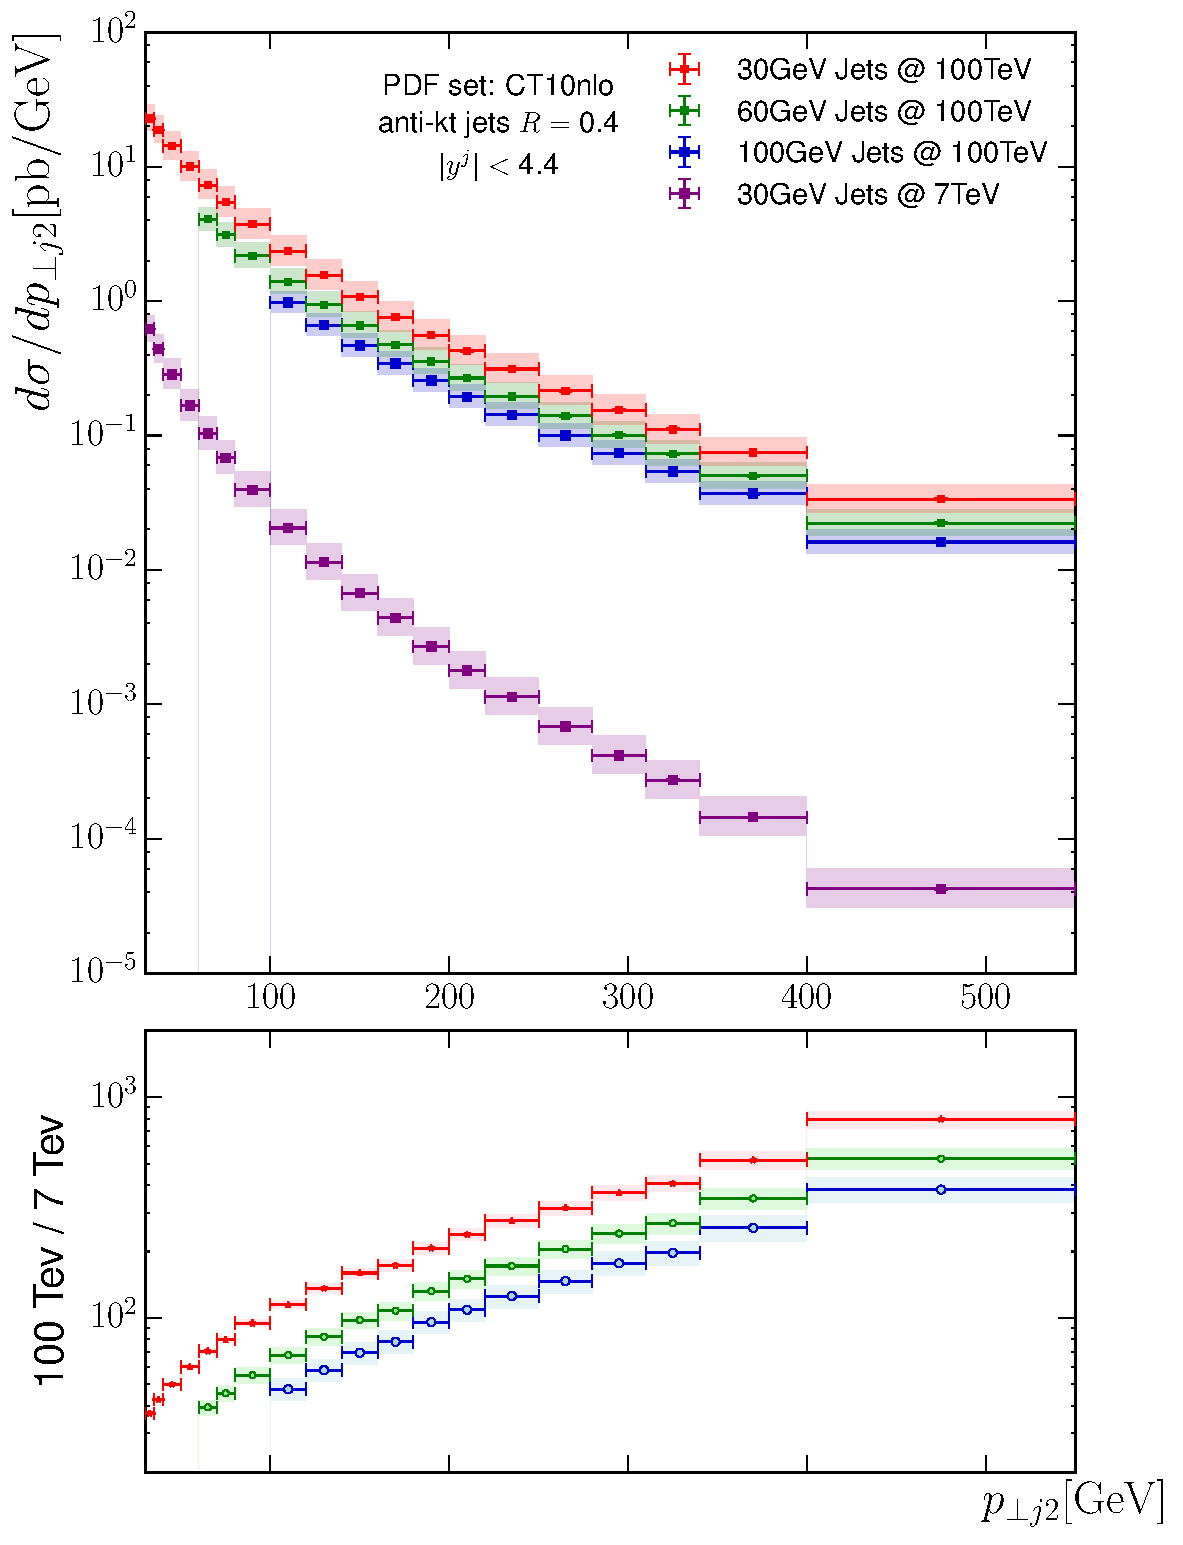
\includegraphics[width=0.8\linewidth]{Figures/ATLAS_Z_100TeV_5b.pdf}
		\caption{5b}
		\label{fig:emissionsites}
	\end{figure}

	\begin{figure}[h]
		\centering
		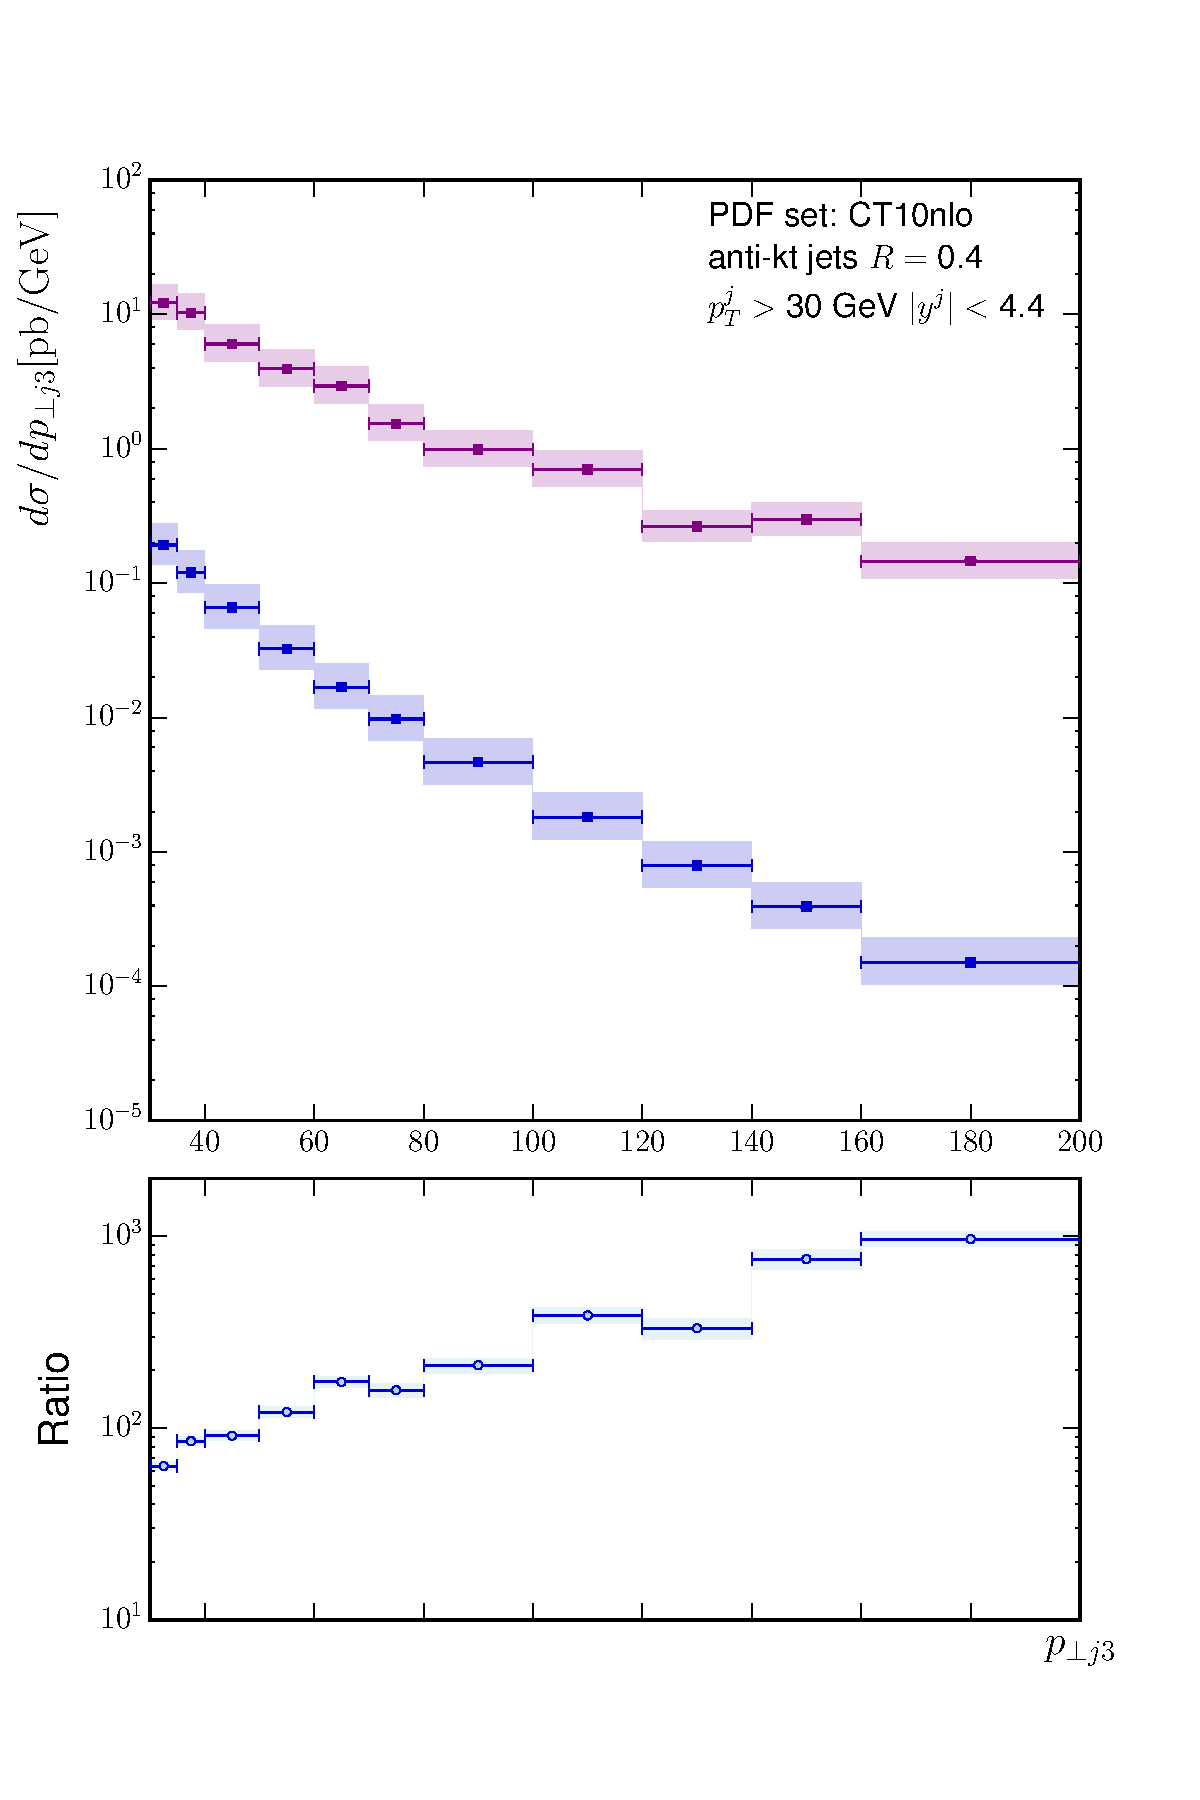
\includegraphics[width=0.8\linewidth]{Figures/ATLAS_Z_100TeV_6a.pdf}
		\caption{6a}
		\label{fig:emissionsites}
	\end{figure}

	\begin{figure}[h]
		\centering
		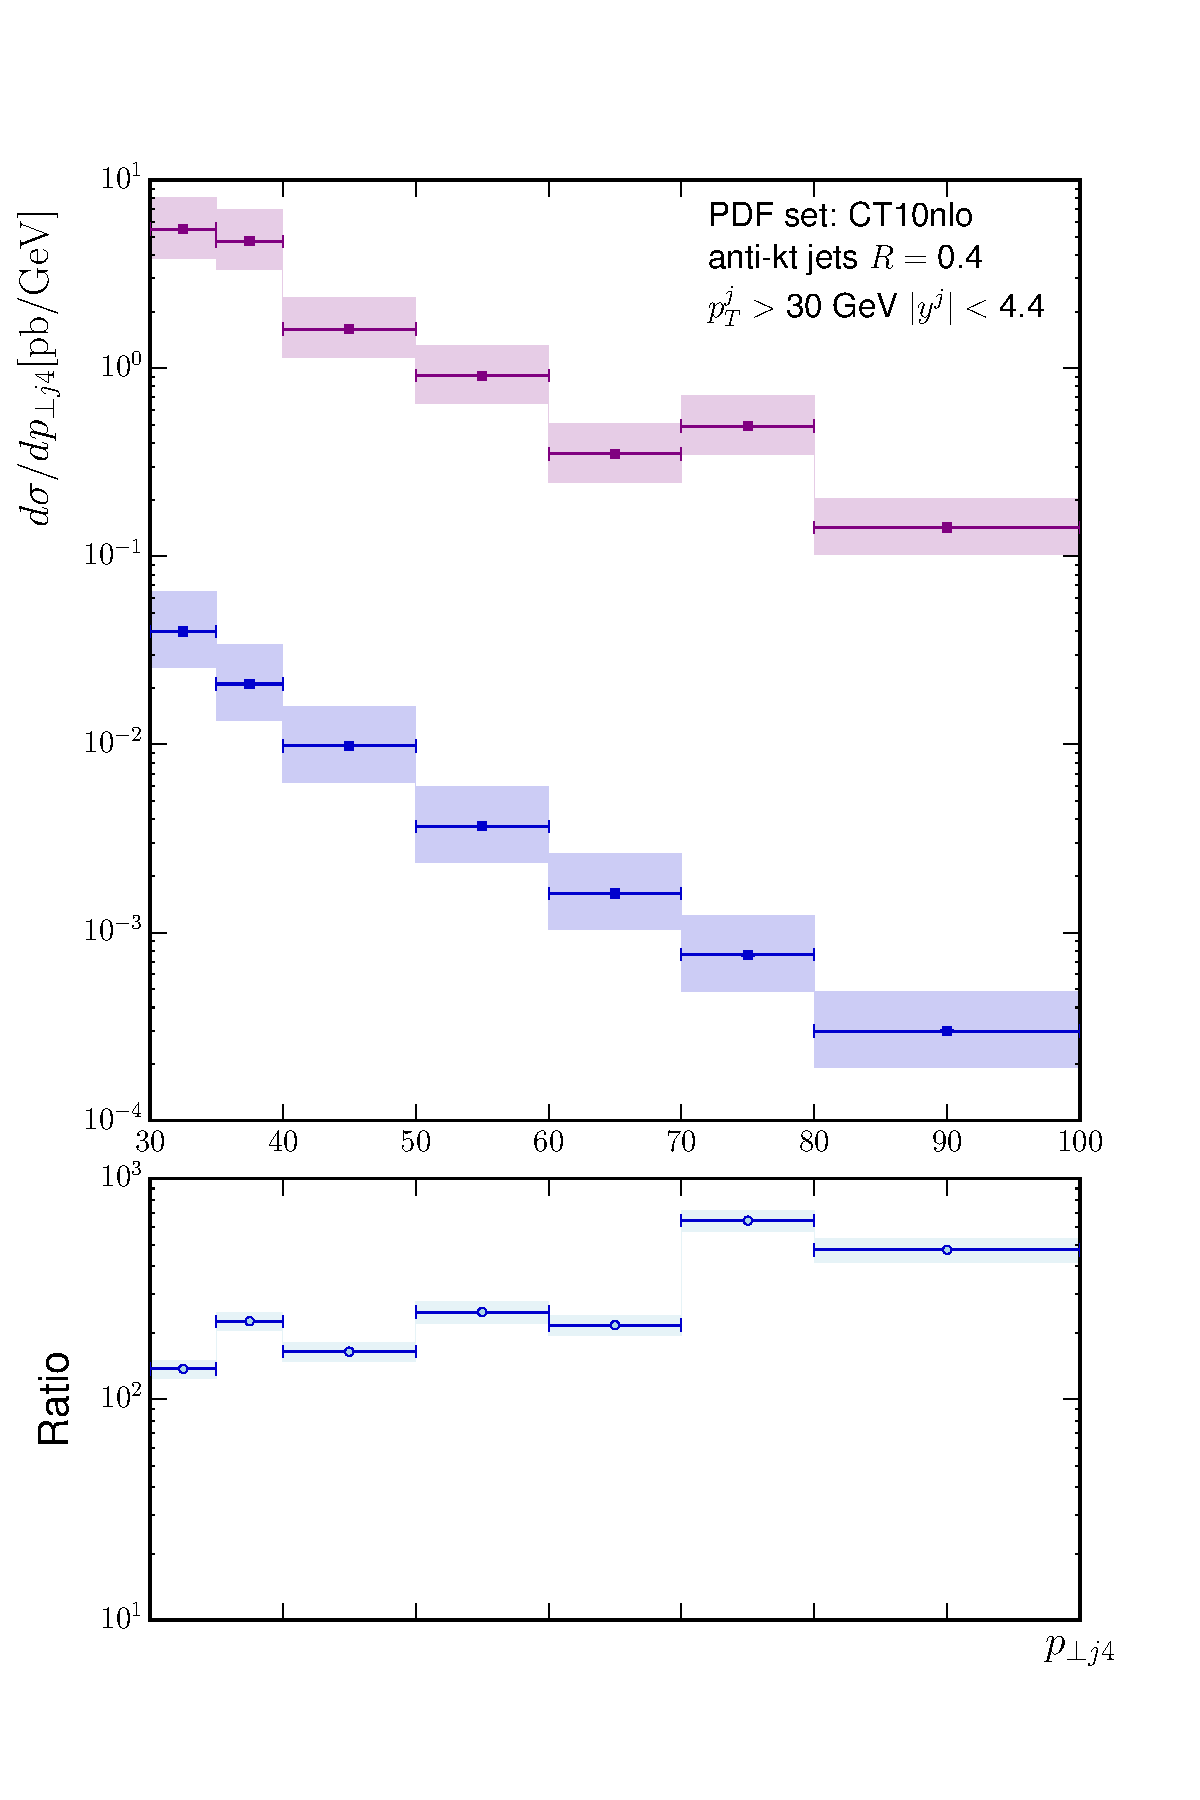
\includegraphics[width=0.8\linewidth]{Figures/ATLAS_Z_100TeV_6b.pdf}
		\caption{6b}
		\label{fig:emissionsites}
	\end{figure}

	\begin{figure}[h]
		\centering
		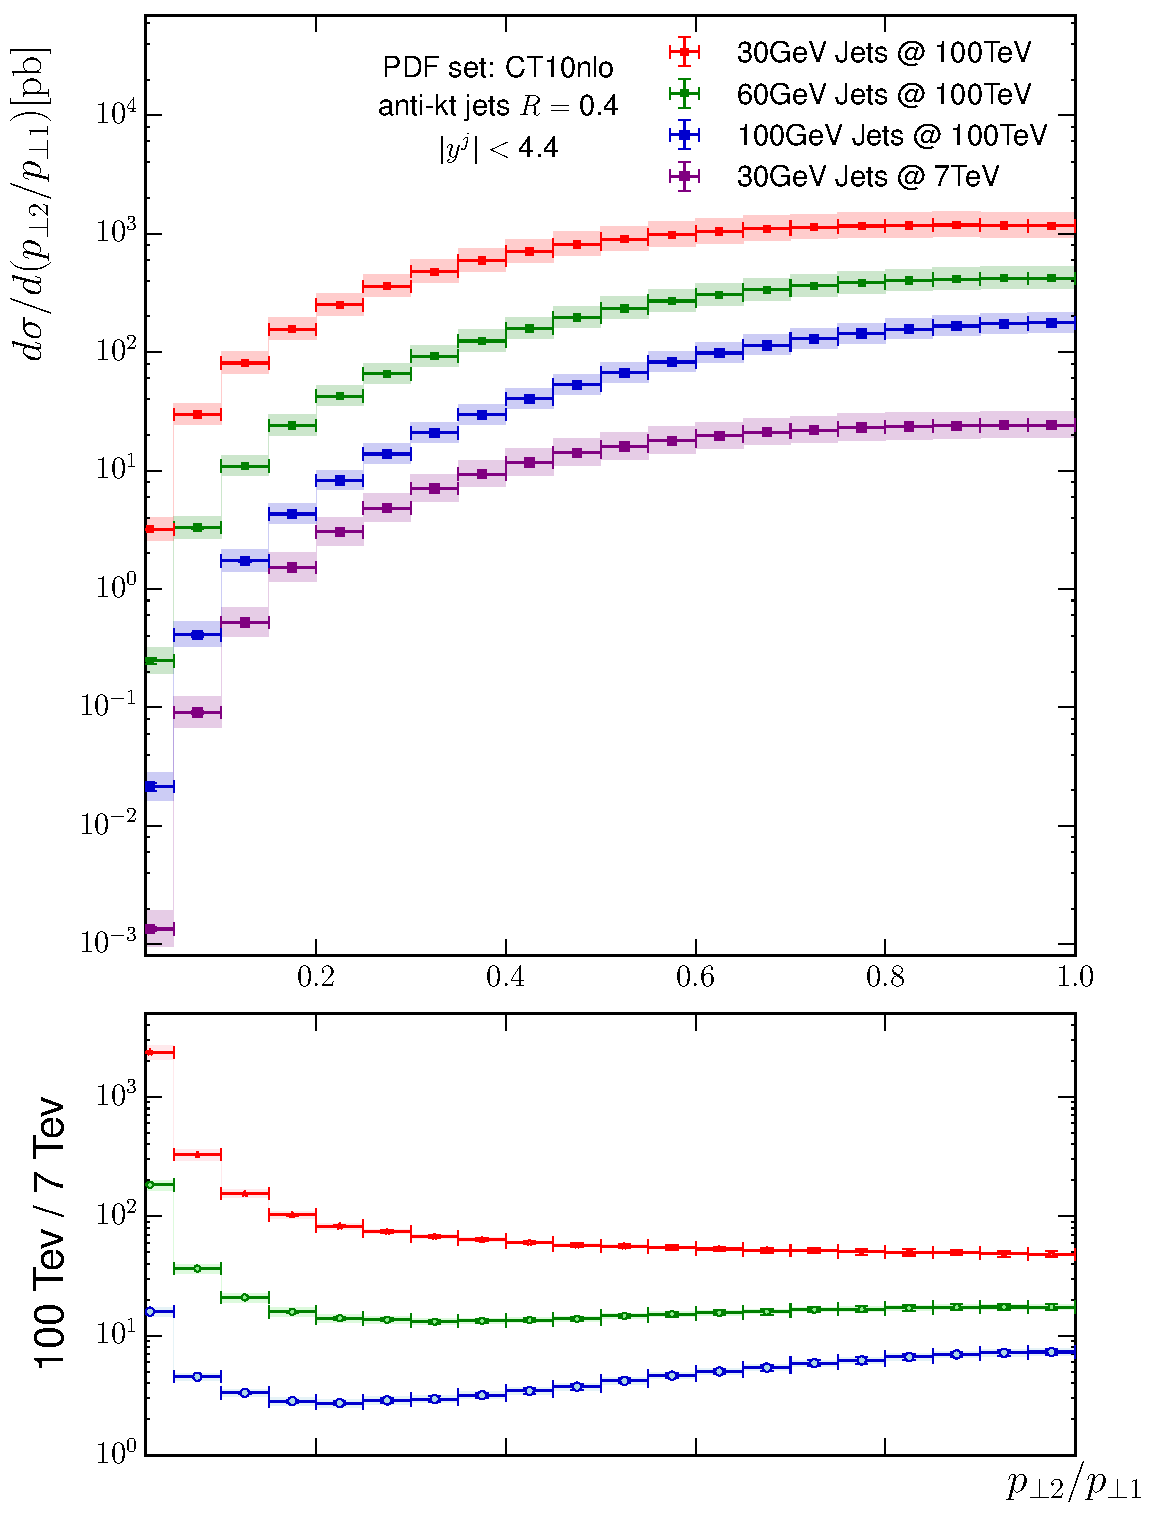
\includegraphics[width=0.8\linewidth]{Figures/ATLAS_Z_100TeV_7b.pdf}
		\caption{7b}
		\label{fig:emissionsites}
	\end{figure}

	\begin{figure}[h]
		\centering
		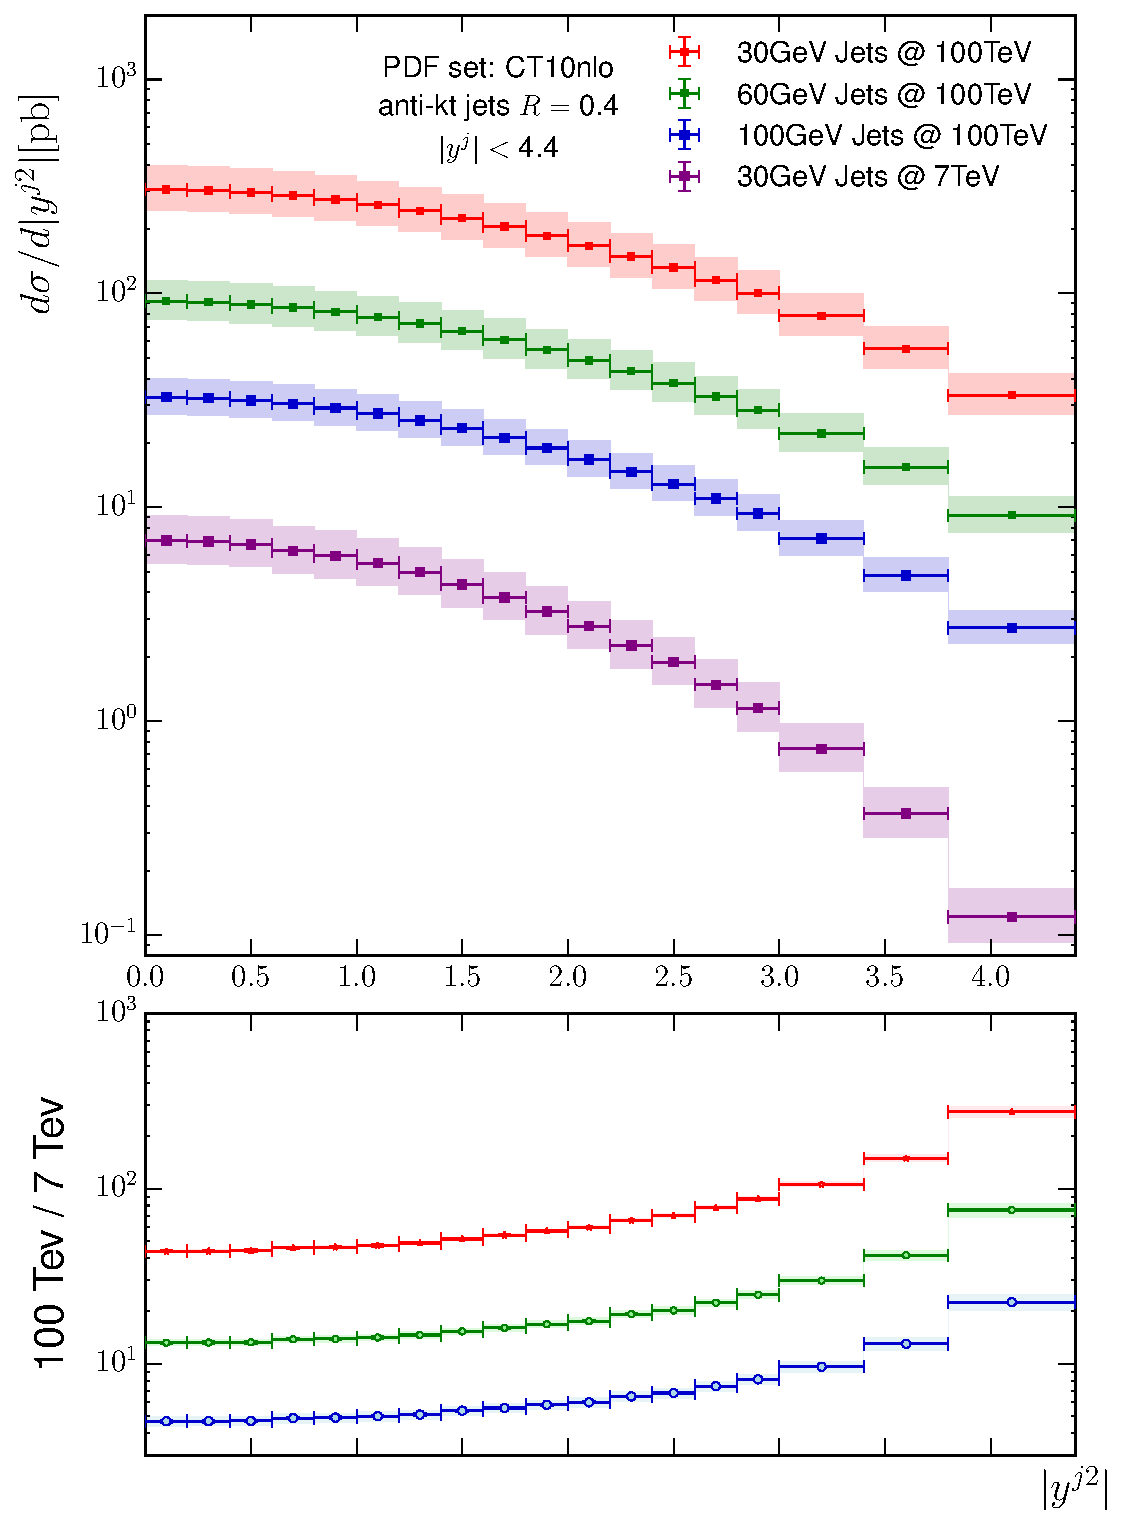
\includegraphics[width=0.8\linewidth]{Figures/ATLAS_Z_100TeV_9b.pdf}
		\caption{9b}
		\label{fig:emissionsites}
	\end{figure}

	\begin{figure}[h]
		\centering
		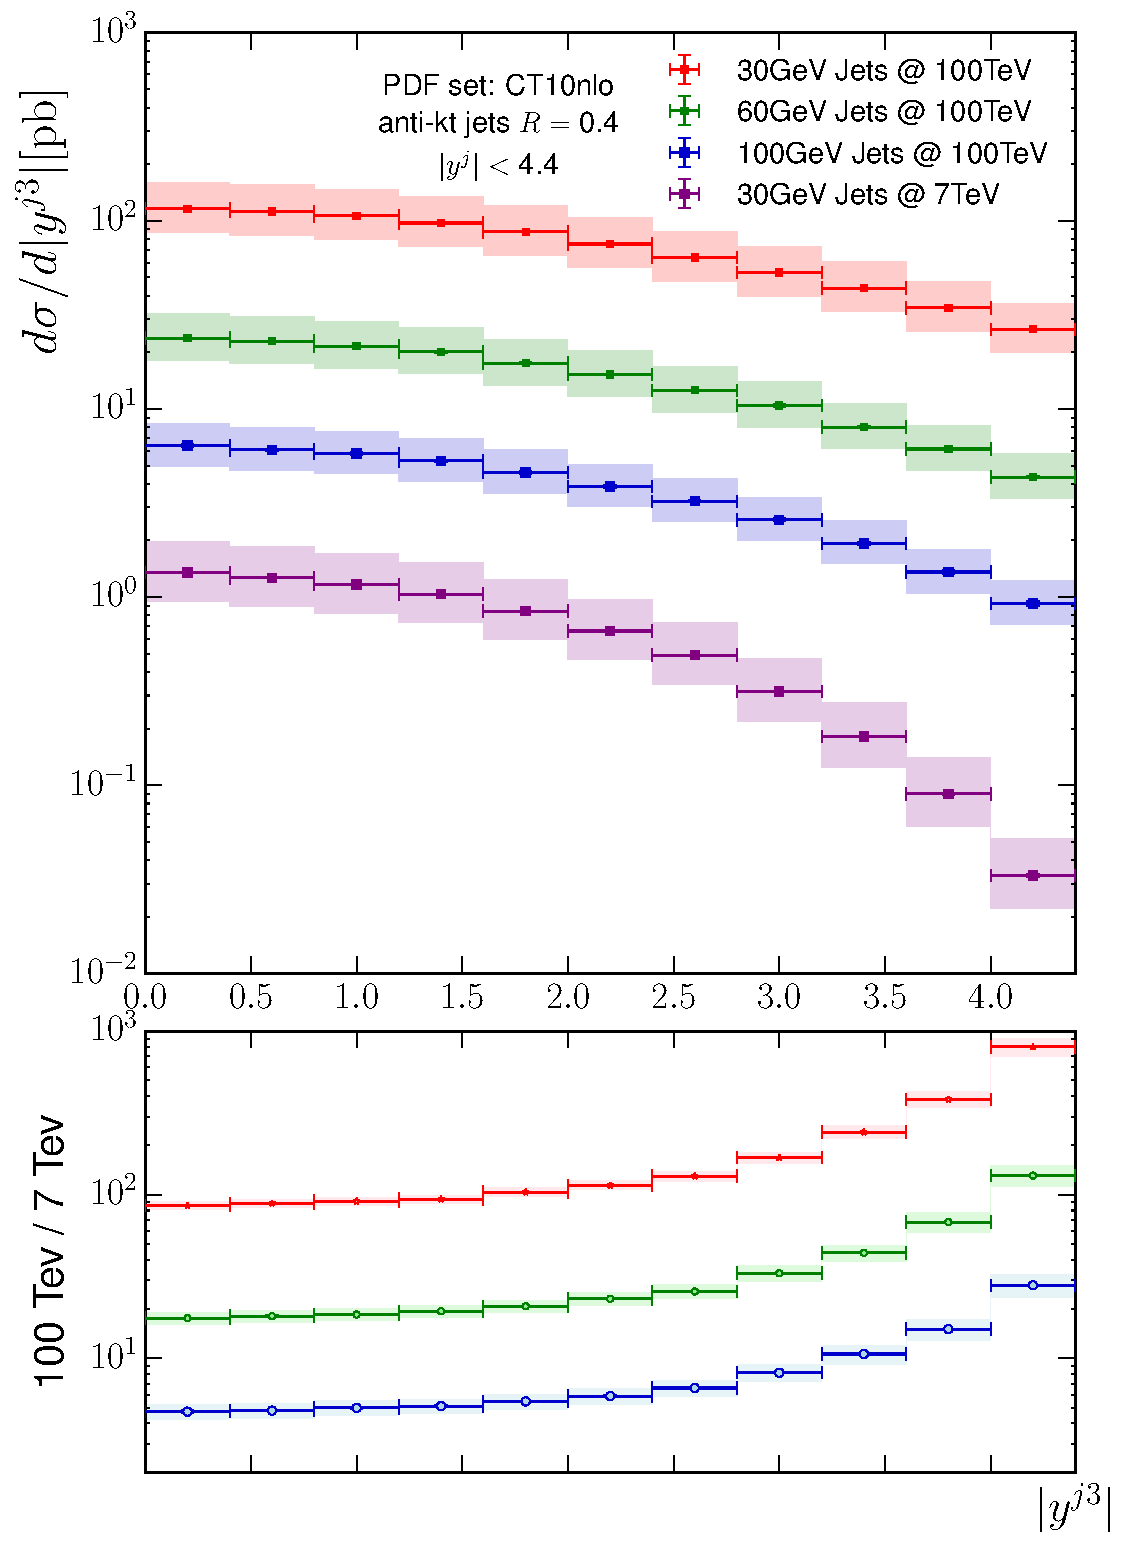
\includegraphics[width=0.8\linewidth]{Figures/ATLAS_Z_100TeV_10a.pdf}
		\caption{10a}
		\label{fig:emissionsites}
	\end{figure}

	\begin{figure}[h]
		\centering
		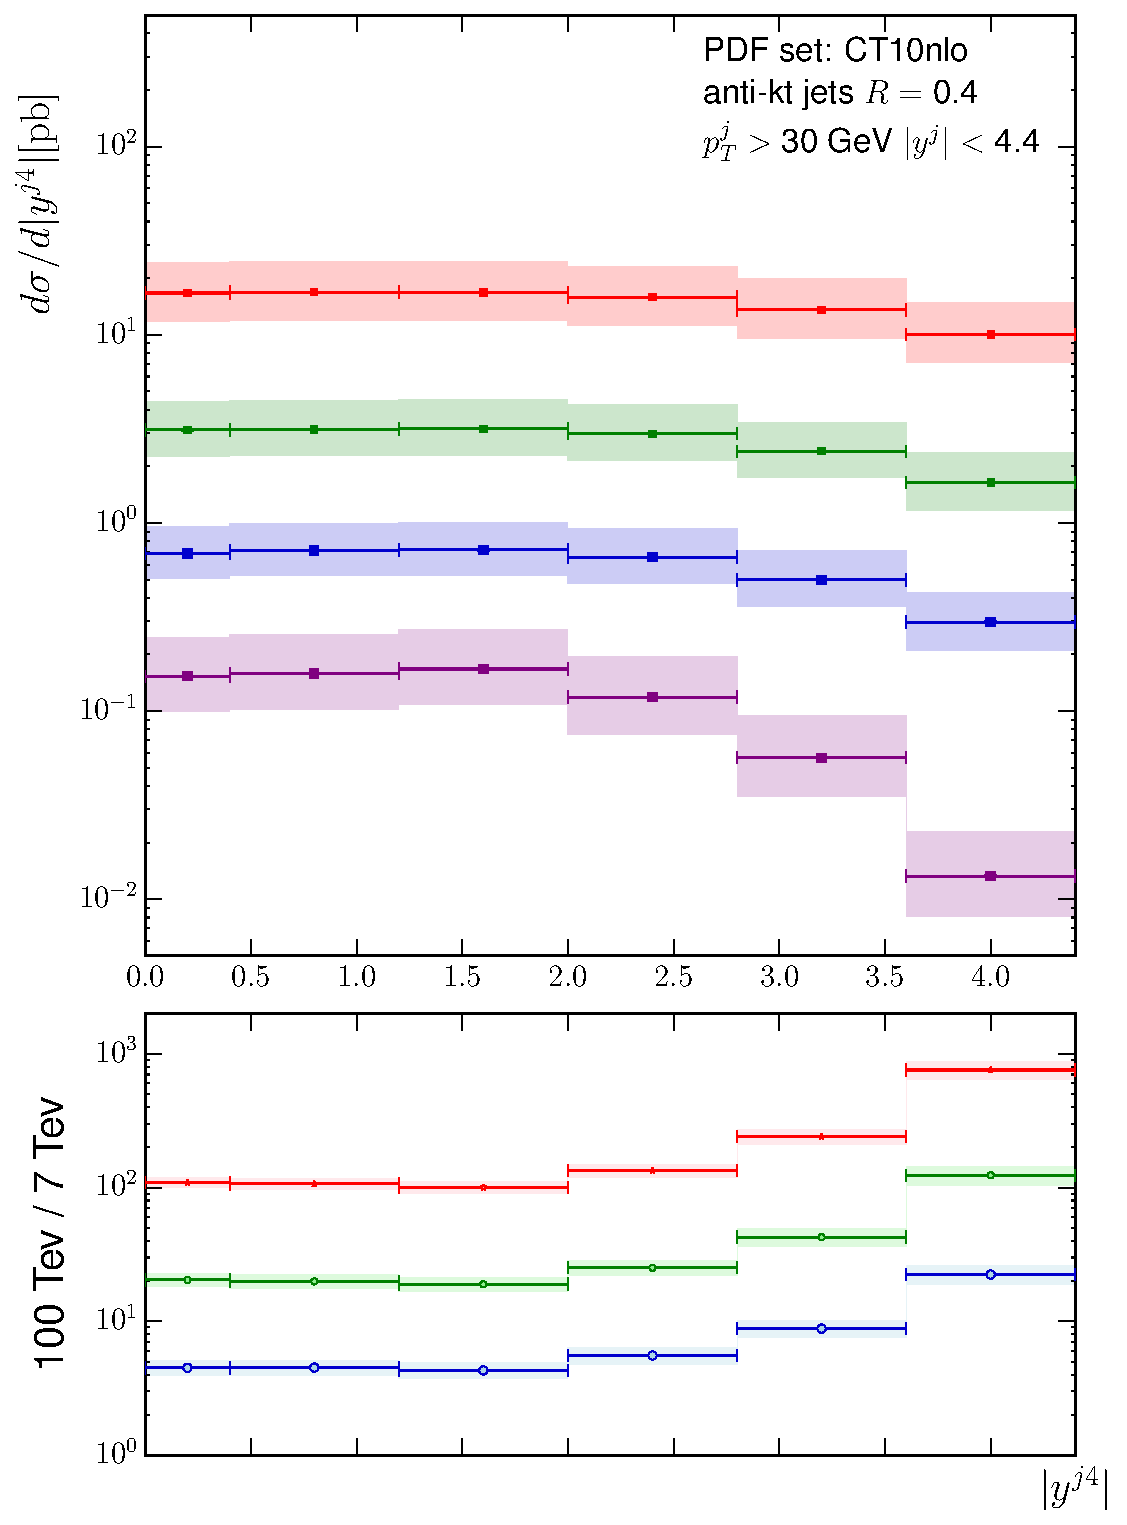
\includegraphics[width=0.8\linewidth]{Figures/ATLAS_Z_100TeV_10b.pdf}
		\caption{10b}
		\label{fig:emissionsites}
	\end{figure}

	\begin{figure}[h]
		\centering
		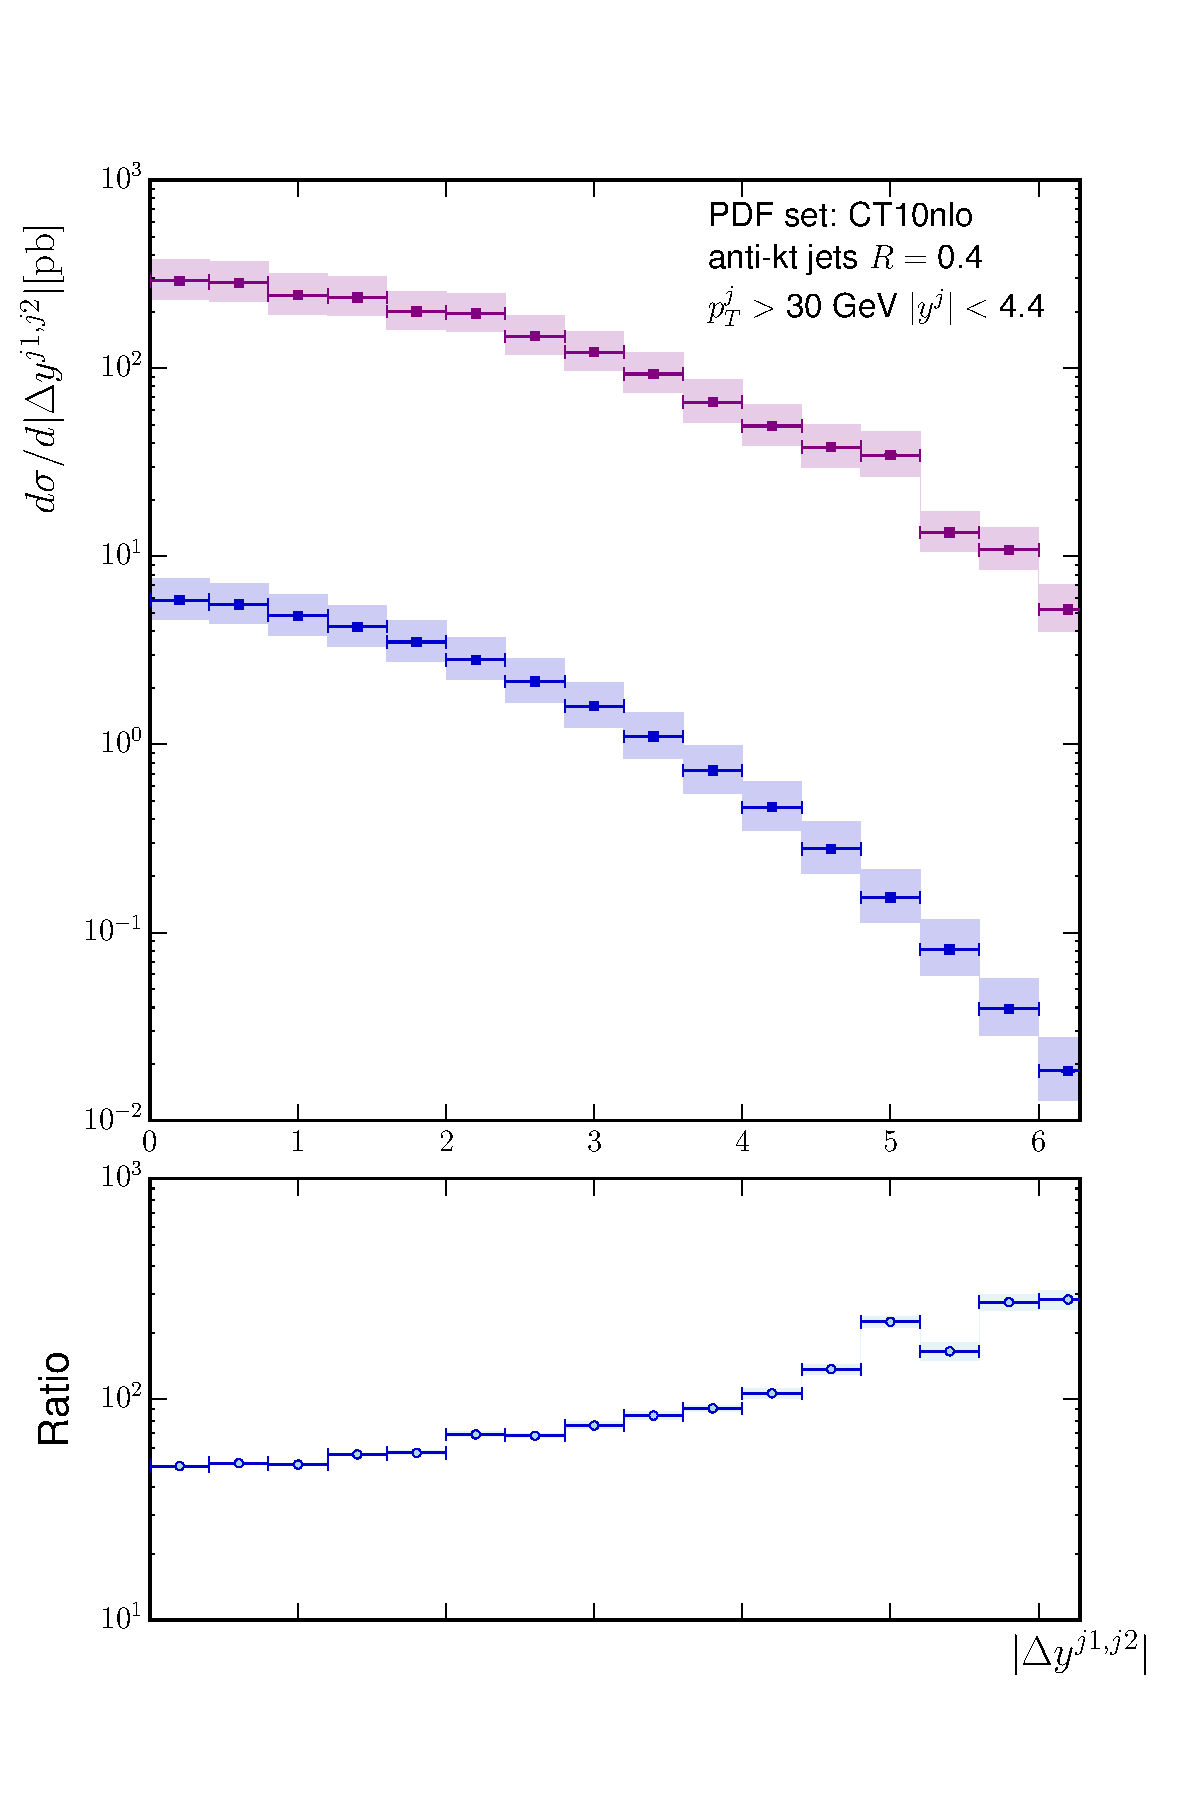
\includegraphics[width=0.8\linewidth]{Figures/ATLAS_Z_100TeV_11a.pdf}
		\caption{11a}
		\label{fig:emissionsites}
	\end{figure}

	\begin{figure}[h]
		\centering
		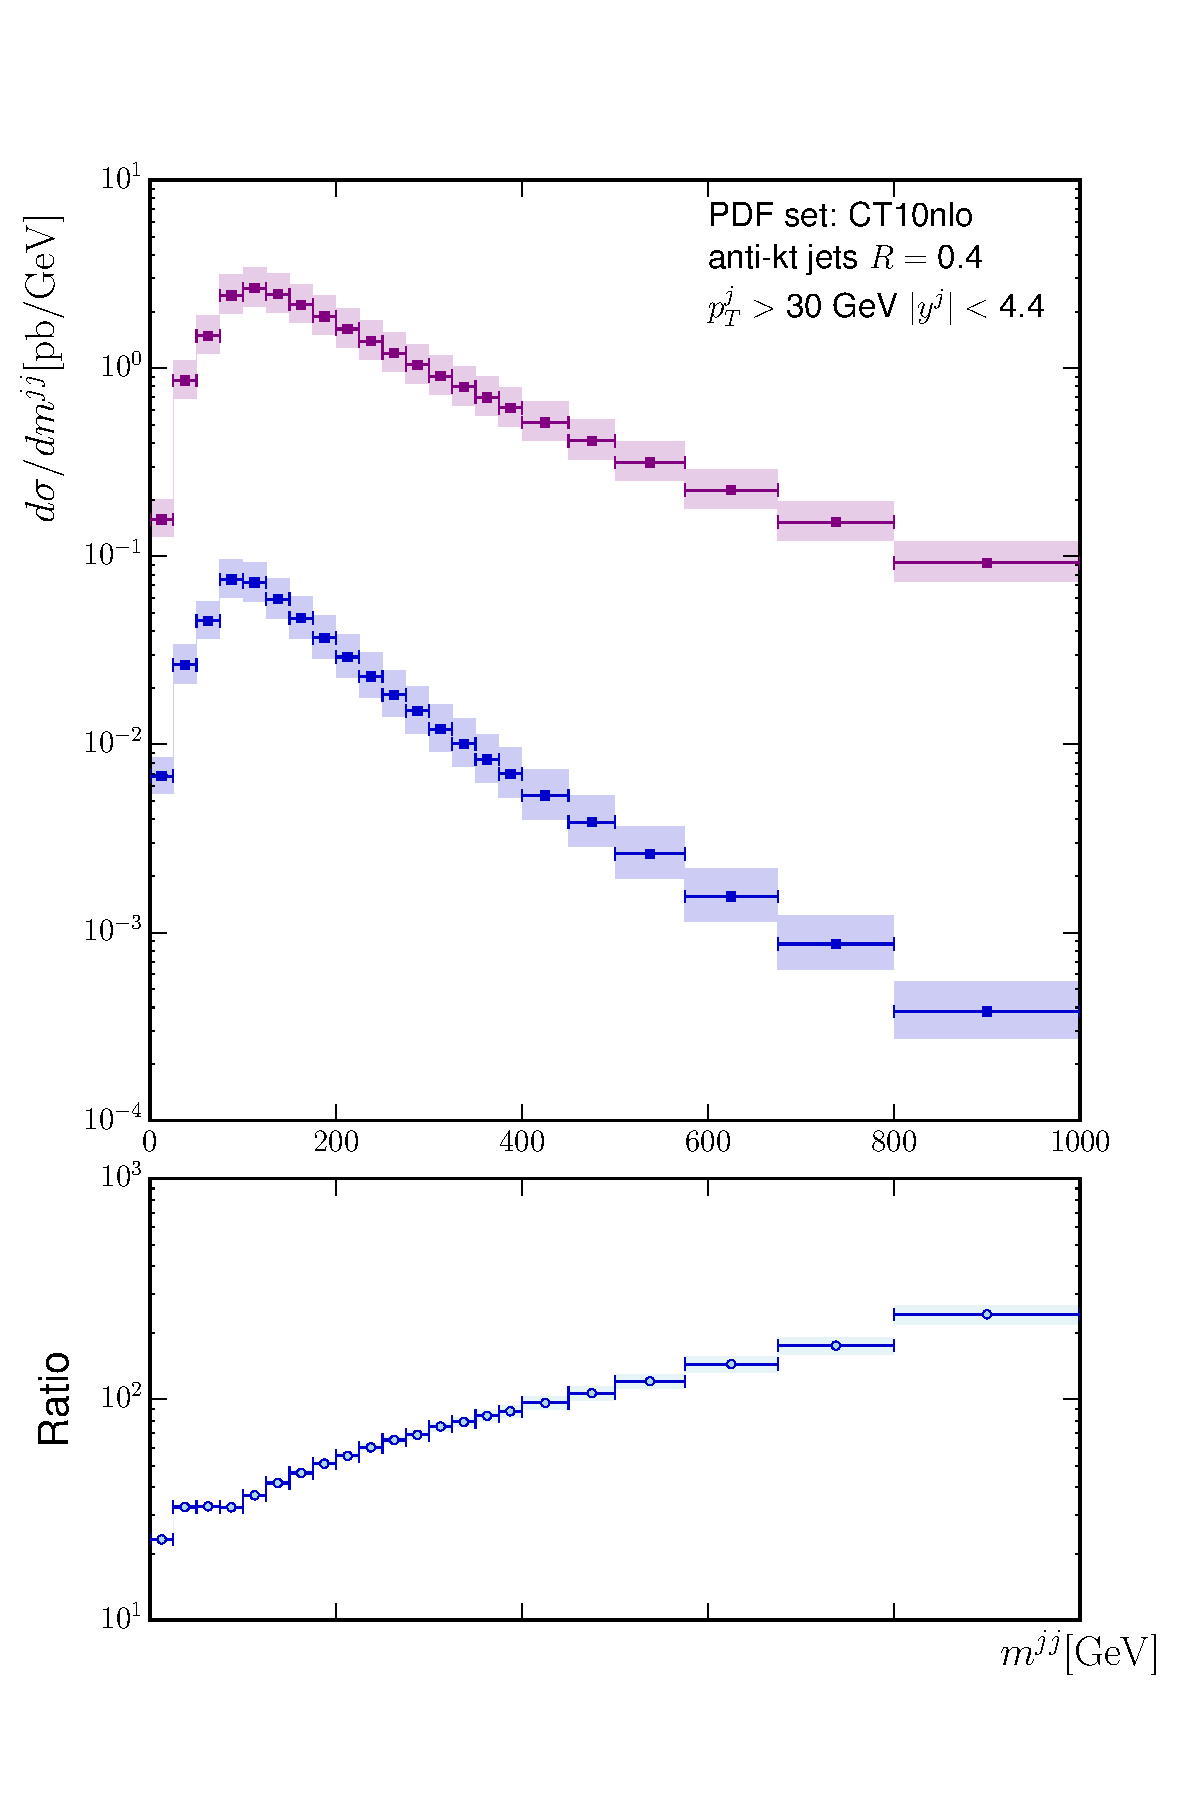
\includegraphics[width=0.8\linewidth]{Figures/ATLAS_Z_100TeV_11b.pdf}
		\caption{11b}
		\label{fig:emissionsites}
	\end{figure}

	\begin{figure}[h]
		\centering
		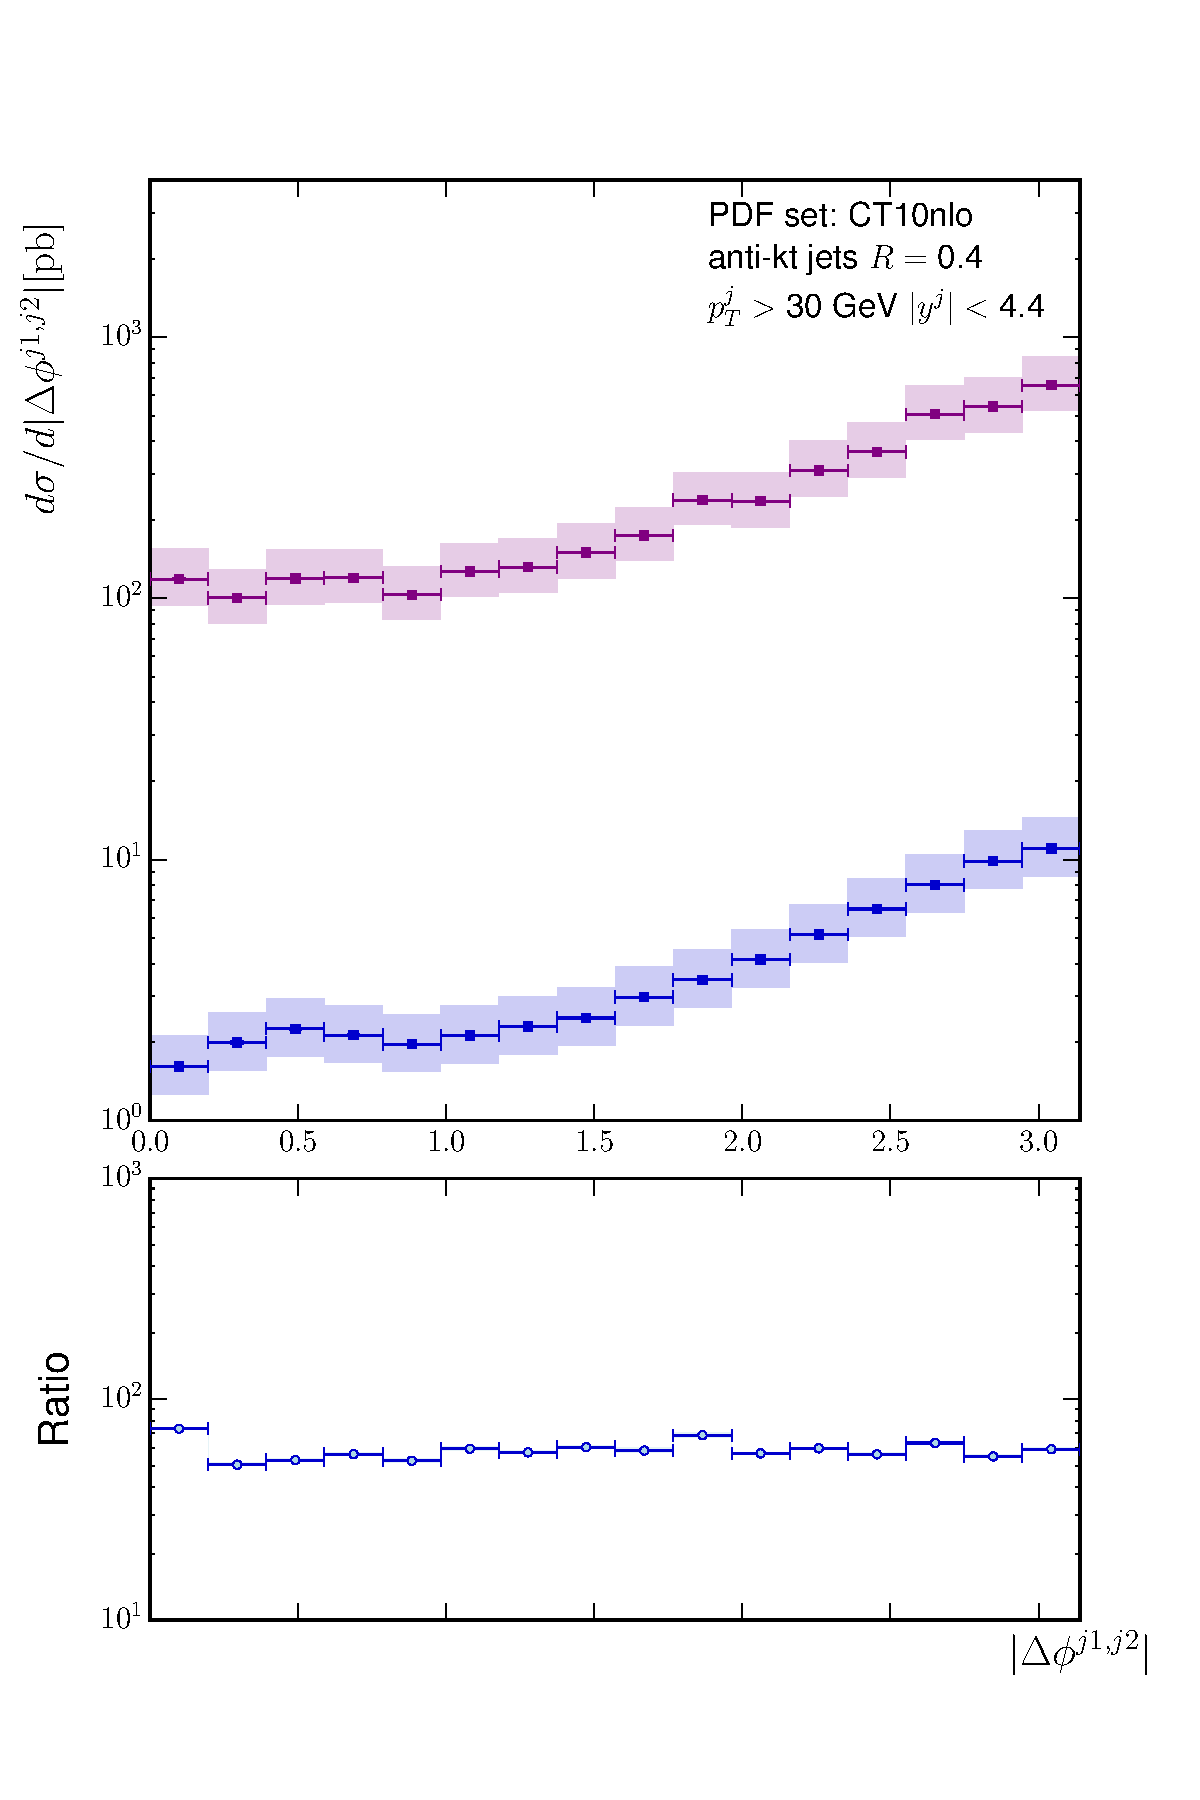
\includegraphics[width=0.8\linewidth]{Figures/ATLAS_Z_100TeV_12a.pdf}
		\caption{12a}
		\label{fig:emissionsites}
	\end{figure}

	\begin{figure}[h]
		\centering
		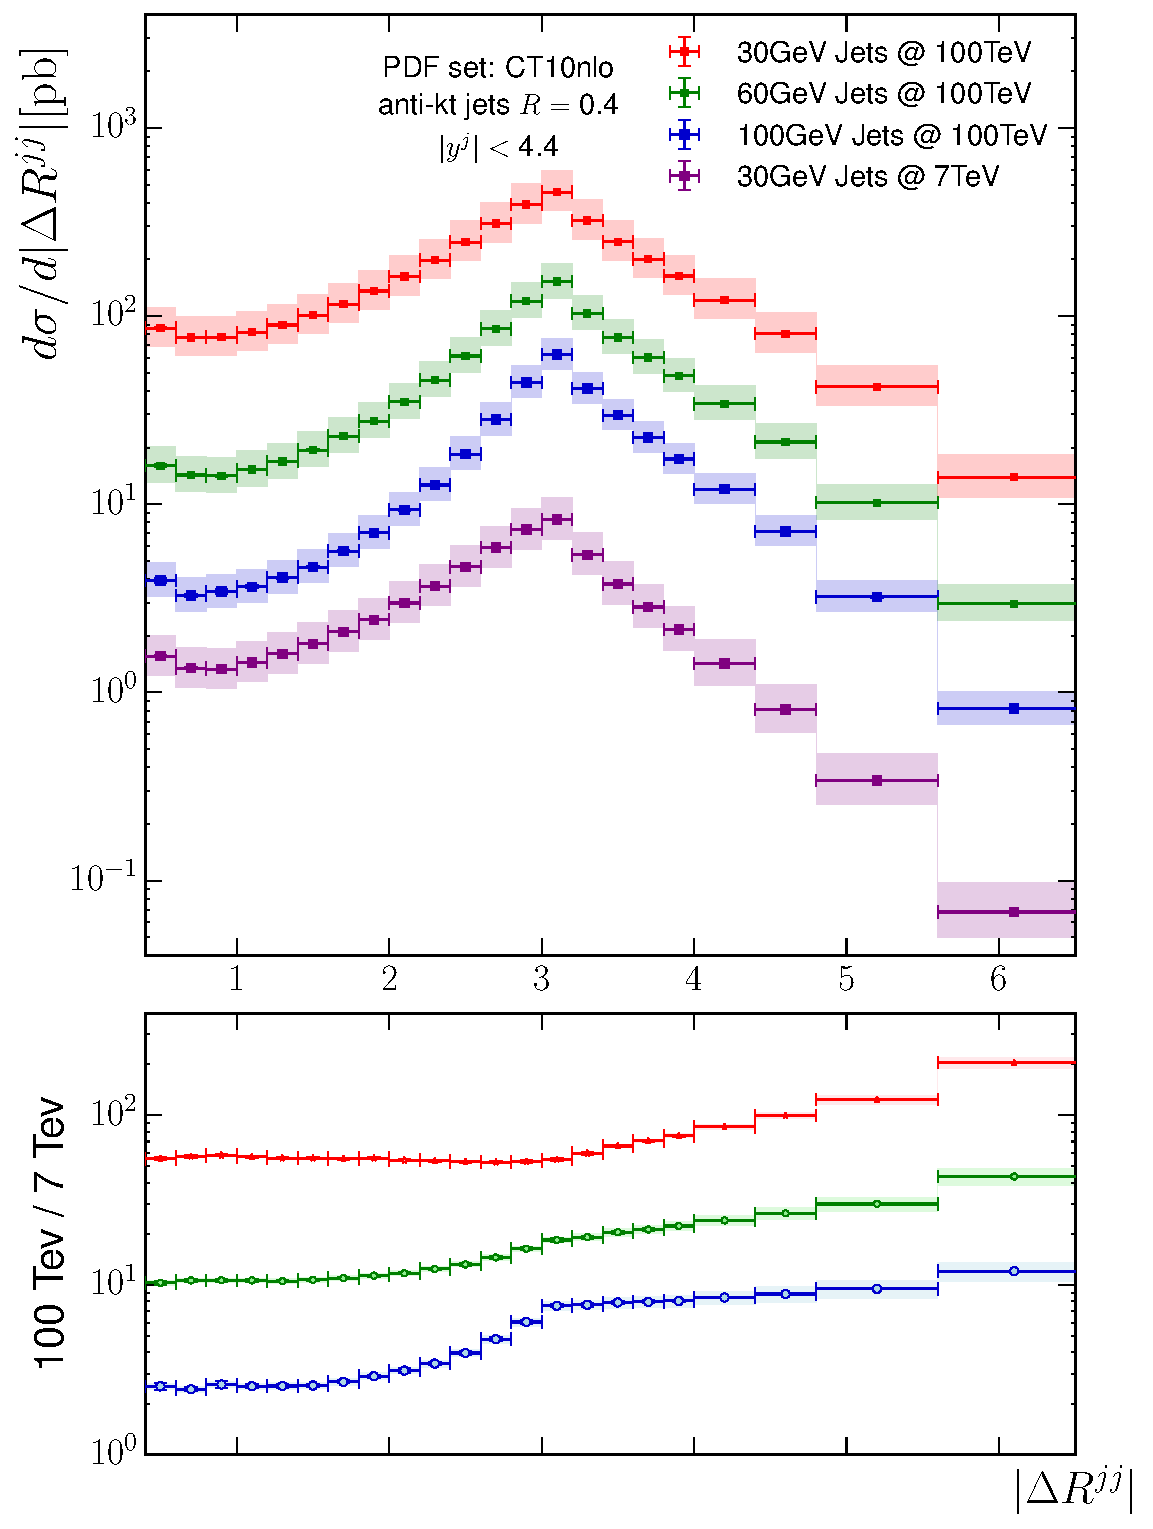
\includegraphics[width=0.8\linewidth]{Figures/ATLAS_Z_100TeV_12b.pdf}
		\caption{12b}
		\label{fig:emissionsites}
	\end{figure}

